
% Sezione con i comandi per CREARE le tabelle.
% Note per noi:
% - Le tabelle Vendita e Acquisto non hanno rispettivamente Cliente e Fornitore perchè i loro riferimenti sono già negli attributi Destinatario e Emittente della relativa Fattura

\vspace{1cm} % spazio bianco
% NOTA: gli spazi sotto sono degli spazi, non TAB, altrimenti non si vedono sul pdf
\begin{verbatim}
create table Cliente (
  Codice VARCHAR(16) primary key,
  Tipo VARCHAR(7) not null,
  IndirizzoPEC VARCHAR(45),
  Nome VARCHAR(45) not null,
  Email VARCHAR(45),
  Via VARCHAR(45),
  NumCivico VARCHAR(11),
  Citta VARCHAR(45),
  CAP INT(11),
  check(Tipo='privato' or Tipo='pa')
)ENGINE=InnoDB;
\end{verbatim}
\vspace{0.5cm}

\noindent\makebox[\textwidth]{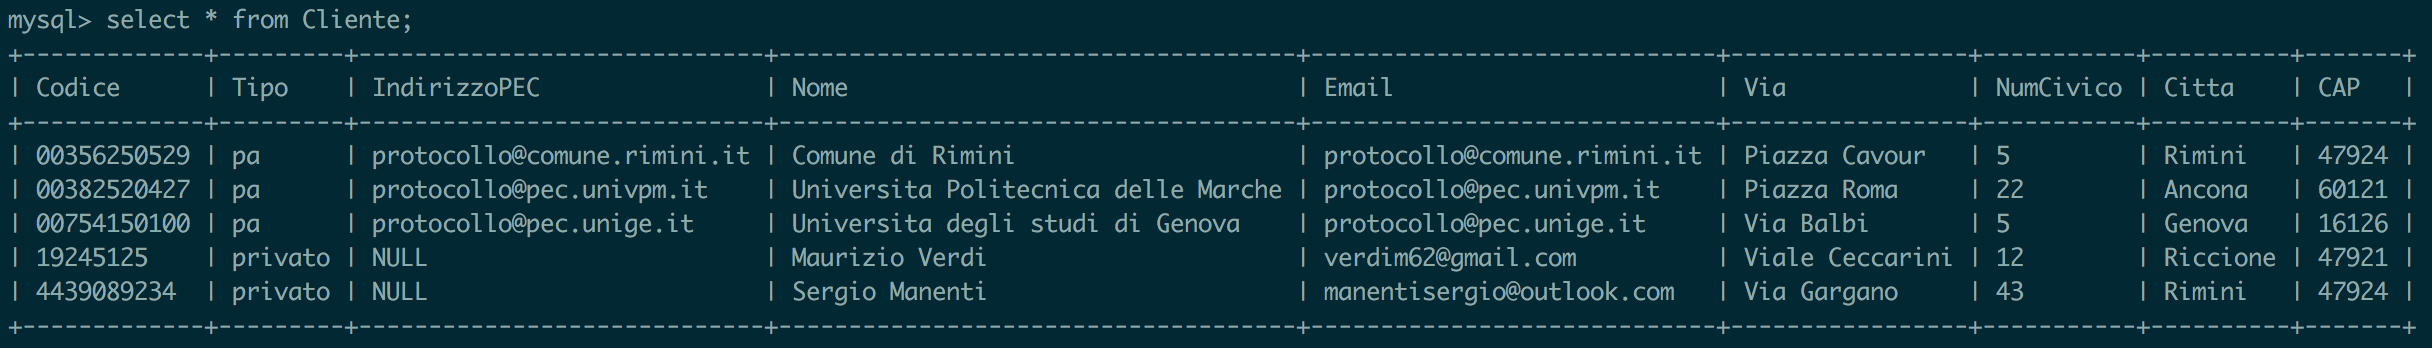
\includegraphics[width=1.2\linewidth]{./immagini/1}}
\newline\newline

\begin{verbatim}
create table RichiestaMEPA (
  Numero INT(11) primary key,
  CodicePA VARCHAR(11) not null,
  OffertaProposta FLOAT(8,2) not null,
  LimiteSpesa FLOAT(8,2) not null,
  InizioOfferte DATE not null,
  TermineOfferte DATE not null,
  foreign key (CodicePA) references Cliente(Codice)
    on update cascade on delete no action,
  check(TermineOfferte > InizioOfferte)
)ENGINE=InnoDB;
\end{verbatim}
\vspace{0.5cm}

\noindent\makebox[\textwidth]{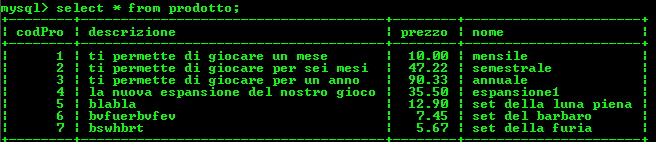
\includegraphics[width=\linewidth]{./immagini/2}}
\newline\newline

\begin{verbatim}
create table Gara (
  RichiestaMEPA INT(11) primary key,
  Aggiudicatario VARCHAR(45),
  OffertaVincitore FLOAT(8,2),
  foreign key (RichiestaMEPA) references RichiestaMEPA(Numero)
    on update cascade on delete cascade
)ENGINE=InnoDB;
\end{verbatim}
\vspace{0.5cm}

\noindent\makebox[\textwidth]{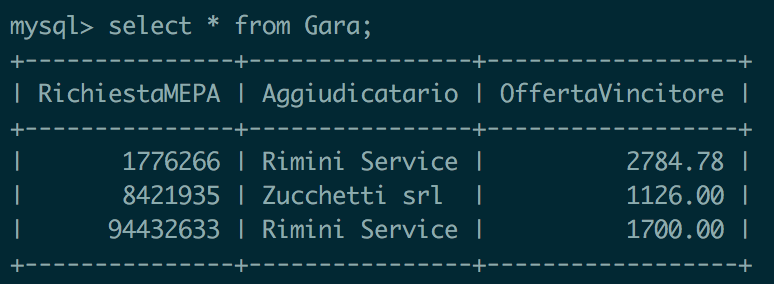
\includegraphics[width=0.7\linewidth]{./immagini/3}}
\newline\newline

\begin{verbatim}
create table Trattativa (
  RichiestaMEPA INT(11) primary key,
  Stipulata BOOLEAN,
  foreign key (RichiestaMEPA) references RichiestaMEPA(Numero)
    on update cascade on delete cascade
)ENGINE=InnoDB;
\end{verbatim}
\vspace{0.5cm}

\noindent\makebox[\textwidth]{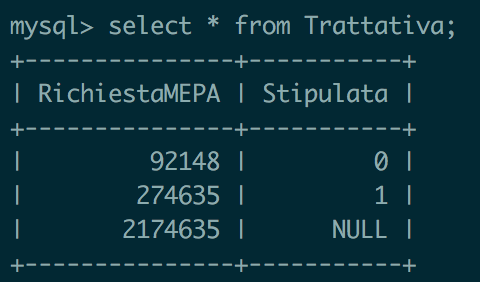
\includegraphics[width=0.5\linewidth]{./immagini/4}}
\newline\newline

\begin{verbatim}
create table Fornitore (
  Codice VARCHAR(16) primary key,
  IndirizzoPEC VARCHAR(45),
  Nome VARCHAR(45) not null,
  Email VARCHAR(45),
  Via VARCHAR(45),
  NumCivico VARCHAR(11),
  Citta VARCHAR(45),
  CAP INT(11)
)ENGINE=InnoDB;
\end{verbatim}
\vspace{0.5cm}

\noindent\makebox[\textwidth]{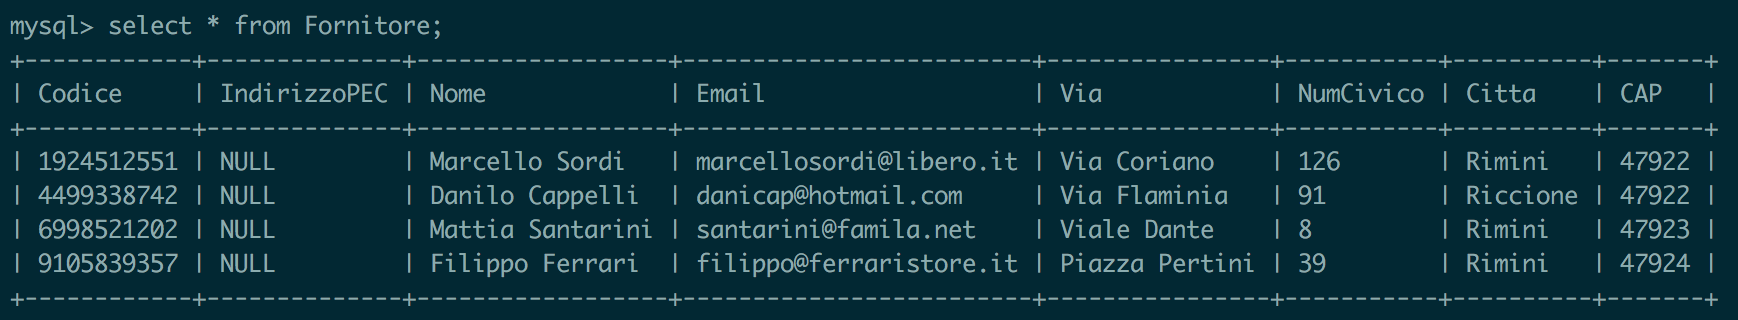
\includegraphics[width=\linewidth]{./immagini/5}}
\newline\newline

\begin{verbatim}
create table TelefonoCliente (
  Numero VARCHAR(11) primary key,
  Cliente VARCHAR(16) not null,
  foreign key (Cliente) references Cliente(Codice)
    on update cascade on delete cascade
)ENGINE=InnoDB;
\end{verbatim}
\vspace{0.5cm}

\noindent\makebox[\textwidth]{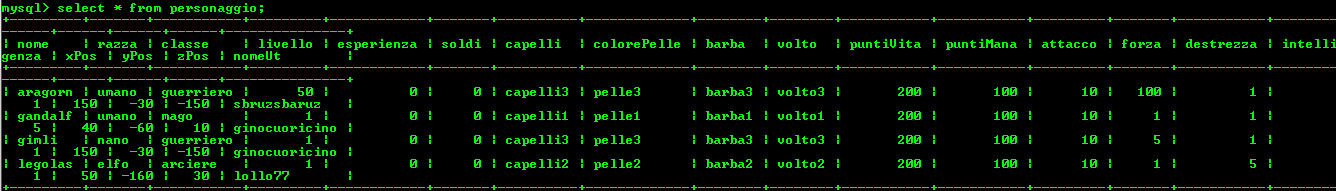
\includegraphics[width=0.6\linewidth]{./immagini/6}}
\newline\newline

\begin{verbatim}
create table TelefonoFornitore (
  Numero VARCHAR(11) primary key,
  Fornitore VARCHAR(16) not null,
  foreign key (Fornitore) references Fornitore(Codice)
    on update cascade on delete cascade
)ENGINE=InnoDB;
\end{verbatim}
\vspace{0.5cm}

\noindent\makebox[\textwidth]{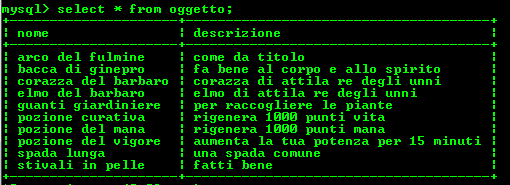
\includegraphics[width=0.7\linewidth]{./immagini/7}}
\newline\newline

\begin{verbatim}
create table CostoSpedizione (
  Codice INT(11) primary key auto_increment,
  Costo FLOAT(8,2) not null,
  Tempo INT(11) not null,
  PesoMax INT(11) not null,
  SommaMisureMax INT(11) not null
)ENGINE=InnoDB;
\end{verbatim}
\vspace{0.5cm}

\noindent\makebox[\textwidth]{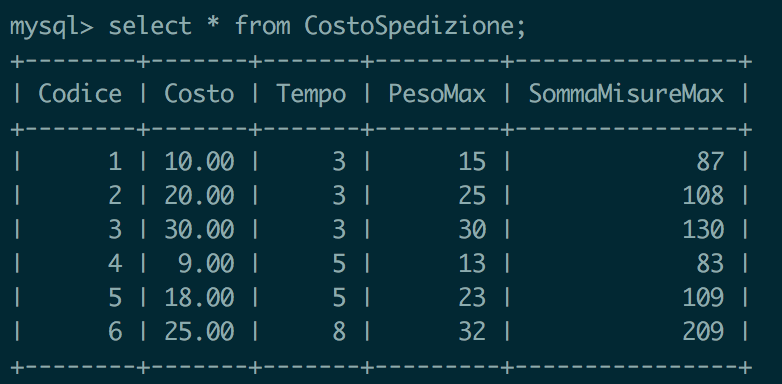
\includegraphics[width=0.7\linewidth]{./immagini/8}}
\newline\newline

\begin{verbatim}
create table Fattura (
  Codice INT(11) primary key auto_increment,
  Emittente VARCHAR(45) not null,
  Destinatario VARCHAR(45) not null,
  Importo FLOAT(8,2),
  Emissione DATE not null,
  Scadenza DATE not null,
  DataPagamento DATE,
  Spedizione INT(11),
  foreign key (Spedizione) references CostoSpedizione(Codice)
    on update cascade on delete no action,
  check (Scadenza > Emissione)
)ENGINE=InnoDB;
\end{verbatim}
\vspace{0.5cm}

\noindent\makebox[\textwidth]{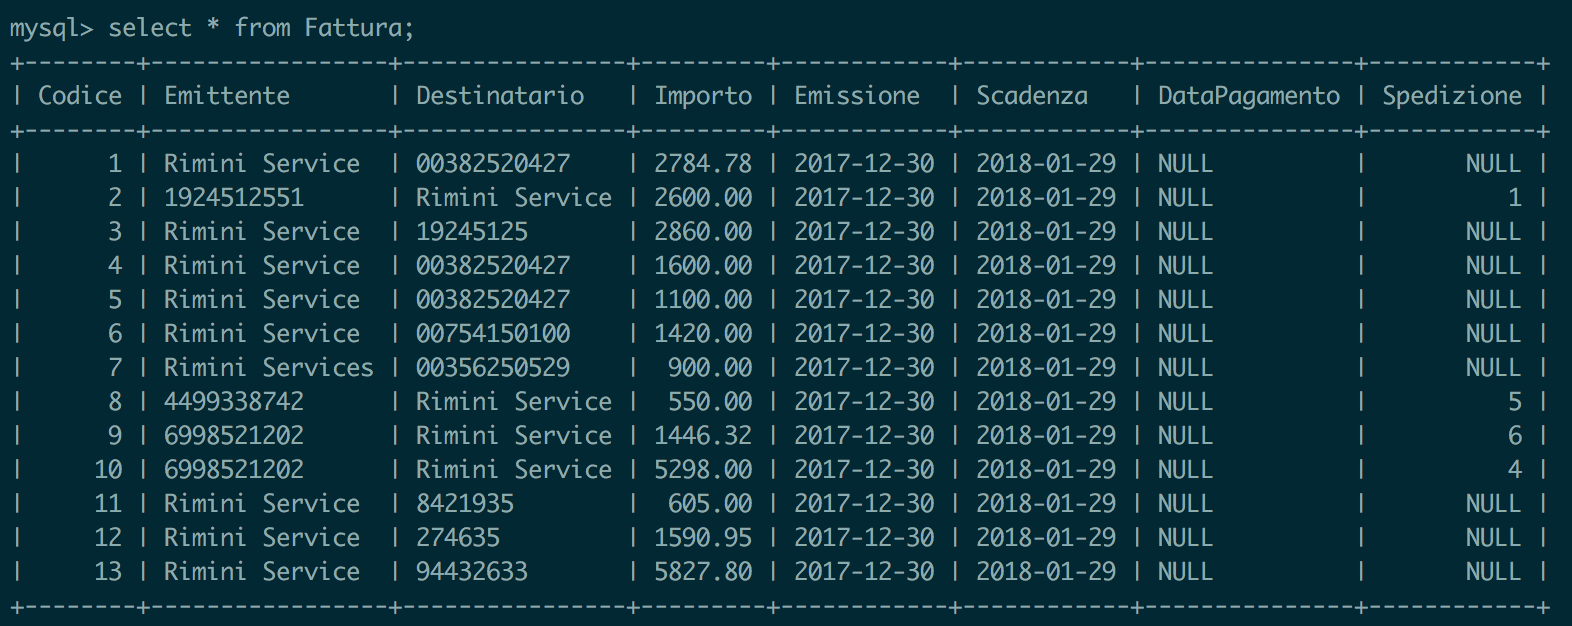
\includegraphics[width=\linewidth]{./immagini/9}}
\newline\newline

\begin{verbatim}
create table ContrattoAssistenza (
  Codice INT(11) primary key auto_increment,
  Importo FLOAT(8,2) not null,
  Cliente VARCHAR(16) not null,
  Inizio DATE not null,
  Termine DATE not null,
  Fattura INT(11) not null,
  foreign key (Cliente) references Cliente(Codice)
    on update cascade on delete no action,
  foreign key (Fattura) references Fattura(Codice)
    on update cascade on delete no action
)ENGINE=InnoDB;
\end{verbatim}
\vspace{0.5cm}

\noindent\makebox[\textwidth]{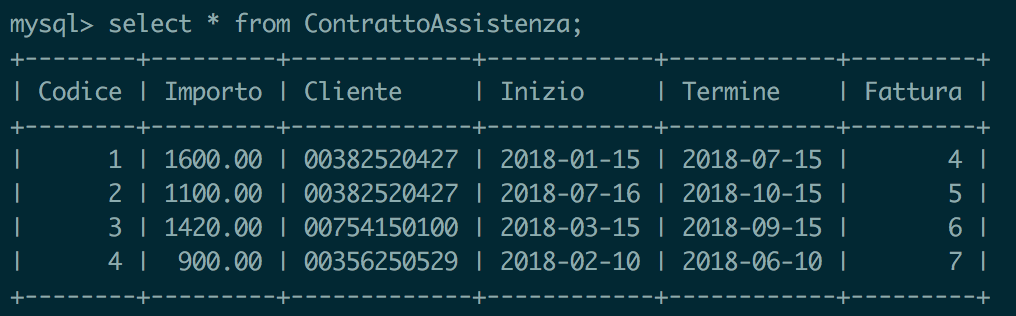
\includegraphics[width=0.8\linewidth]{./immagini/10}}
\newline\newline

\begin{verbatim}
create table ProdottoServizio (
  Codice VARCHAR(20) primary key
)ENGINE=InnoDB;
\end{verbatim}
\vspace{0.5cm}

\noindent\makebox[\textwidth]{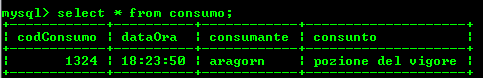
\includegraphics[width=0.5\linewidth]{./immagini/11}}
\newline\newline

\begin{verbatim}
create table Prodotto (
  Codice VARCHAR(20) primary key,
  Produttore VARCHAR(45) not null,
  Modello VARCHAR(45) not null,
  Peso FLOAT(4,1) not null,
  Dimensioni VARCHAR(20) not null,
  foreign key (Codice) references ProdottoServizio(Codice)
    on update cascade on delete cascade
)ENGINE=InnoDB;
\end{verbatim}
\vspace{0.5cm}

\noindent\makebox[\textwidth]{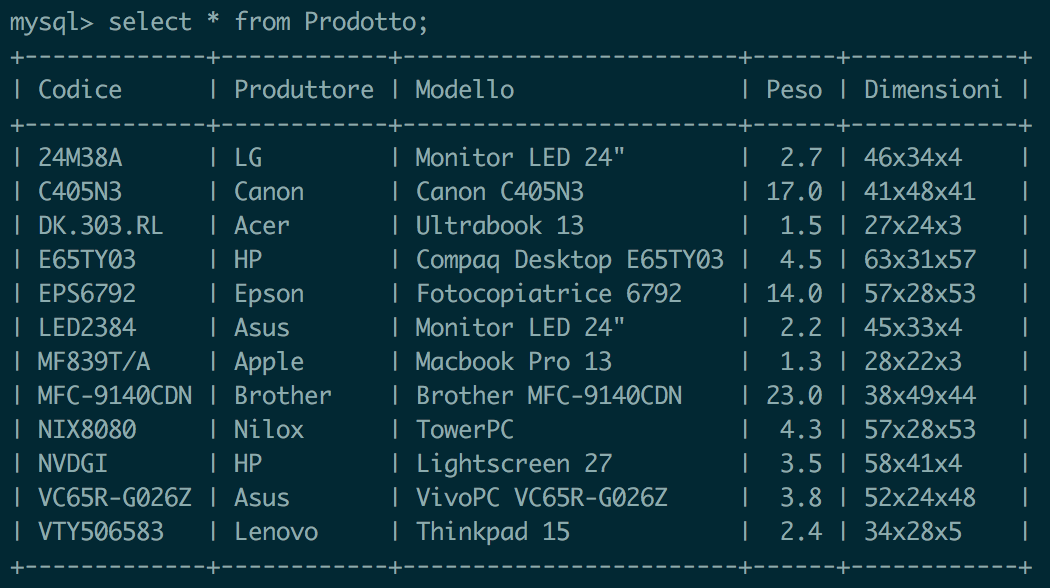
\includegraphics[width=0.8\linewidth]{./immagini/12}}
\newline\newline

\begin{verbatim}
create table Notebook (
  Codice VARCHAR(20) primary key,
  Processore VARCHAR(15) not null,
  RAM INT(11) not null,
  Storage INT(11) not null,
  Schermo FLOAT(3,1) not null,
  SistemaOperativo VARCHAR(45) not null,
  foreign key (Codice) references Prodotto(Codice)
    on update cascade on delete cascade,
  check(SistemaOperativo='Windows 10'
    or SistemaOperativo='Windows 7'
    or SistemaOperativo='Mac OS X'
    or SistemaOperativo='Linux'
    or SistemaOperativo='Free Dos')
)ENGINE=InnoDB;
\end{verbatim}
\vspace{0.5cm}

\noindent\makebox[\textwidth]{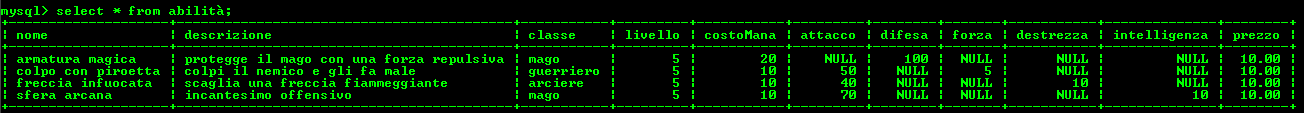
\includegraphics[width=0.8\linewidth]{./immagini/13}}
\newline\newline

\begin{verbatim}
create table PCDesktop (
  Codice VARCHAR(20) primary key,
  Processore VARCHAR(15) not null,
  RAM INT(11) not null,
  Storage INT(11) not null,
  SistemaOperativo VARCHAR(45) not null,
  foreign key (Codice) references Prodotto(Codice)
    on update cascade on delete cascade,
  check(SistemaOperativo='Windows 10'
    or SistemaOperativo='Windows 7'
    or SistemaOperativo='Mac OS X'
    or SistemaOperativo='Linux'
    or SistemaOperativo='Free Dos')
)ENGINE=InnoDB;
\end{verbatim}
\vspace{0.5cm}

\noindent\makebox[\textwidth]{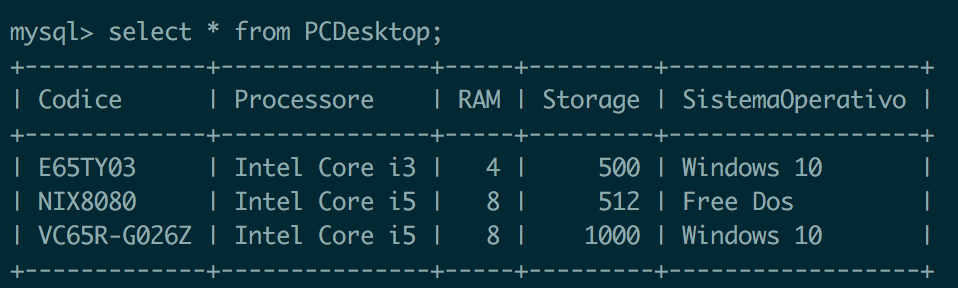
\includegraphics[width=0.8\linewidth]{./immagini/14}}
\newline\newline

\begin{verbatim}
create table Monitor (
  Codice VARCHAR(20) primary key,
  Dimensione FLOAT(3,1) not null,
  Risoluzione VARCHAR(11) not null,
  foreign key (Codice) references Prodotto(Codice)
    on update cascade on delete cascade,
  check(Risoluzione='800x600'
    or Risoluzione='1024x768'
    or Risoluzione='1280x720'
    or Risoluzione='1280x800'
    or Risoluzione='1440x900'
    or Risoluzione='1650x1080'
    or Risoluzione='1920x1080'
    or Risoluzione='1920x1200'
    or Risoluzione='2560x1600')
)ENGINE=InnoDB;
\end{verbatim}
\vspace{0.5cm}

\noindent\makebox[\textwidth]{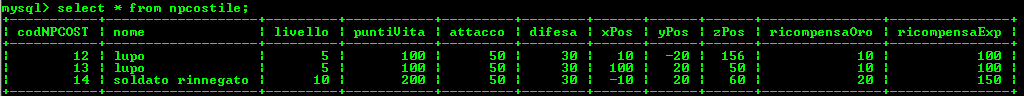
\includegraphics[width=0.6\linewidth]{./immagini/15}}
\newline\newline

\begin{verbatim}
create table Stampante (
  Codice VARCHAR(20) primary key,
  Tecnologia VARCHAR(6) not null,
  FormatoMax CHAR(2) not null,
  Velocita INT(11) not null,
  Connettivita VARCHAR(9) not null,
  foreign key (Codice) references Prodotto(Codice)
    on update cascade on delete cascade,
  check(Tecnologia='Inkjet' or Tecnologia='Laser'),
  check(FormatoMax='A3' or FormatoMax='A4' or FormatoMax='A5'),
  check(Connettivita='USB' or Connettivita='WiFi'
    or Connettivita='USB, WiFi')
)ENGINE=InnoDB;
\end{verbatim}
\vspace{0.5cm}

\noindent\makebox[\textwidth]{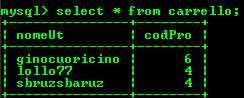
\includegraphics[width=0.8\linewidth]{./immagini/16}}
\newline\newline

\begin{verbatim}
create table Servizio (
  Codice VARCHAR(20) primary key,
  Tipologia VARCHAR(24) not null,
  Costo INT(11) not null,
  foreign key(Codice) references ProdottoServizio(Codice)
    on update cascade on delete cascade,
  check(Tipologia='Riparazione software'
    or Tipologia='Sostituzione componente'
    or Tipologia='Configurazione programma'
    or Tipologia='Formattazione pc'
    or Tipologia='Installazione rete WiFi')
)ENGINE=InnoDB;
\end{verbatim}
\vspace{0.5cm}

\noindent\makebox[\textwidth]{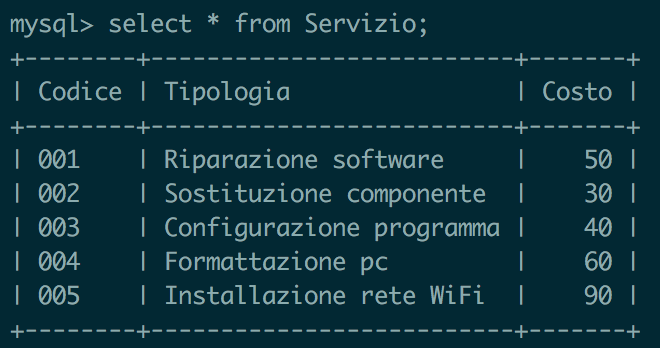
\includegraphics[width=0.7\linewidth]{./immagini/17}}
\newline\newline

\begin{verbatim}
create table Catalogo (
  Fornitore VARCHAR(16) not null,
  Prodotto VARCHAR(20) not null,
  primary key (Fornitore, Prodotto),
  Prezzo FLOAT(8,2) not null,
  InizioValidita DATE not null,
  FineValidita DATE not null,
  foreign key (Fornitore) references Fornitore(Codice)
    on update cascade on delete no action,
  foreign key (Prodotto) references Prodotto(Codice)
    on update cascade on delete no action,
  check (InizioValidita < FineValidita)
)ENGINE=InnoDB;
\end{verbatim}
\vspace{0.5cm}

\noindent\makebox[\textwidth]{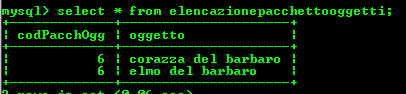
\includegraphics[width=0.8\linewidth]{./immagini/18}}
\newline\newline

\begin{verbatim}
create table ElencazioneCostiSpedizione (
  Fornitore VARCHAR(16),
  Costo INT(11),
  primary key (Fornitore, Costo),
  foreign key (Fornitore) references Fornitore(Codice)
    on update cascade on delete no action,
  foreign key (Costo) references CostoSpedizione(Codice)
    on update cascade on delete no action
)ENGINE=InnoDB;
\end{verbatim}
\vspace{0.5cm}

\noindent\makebox[\textwidth]{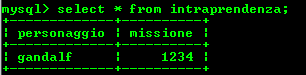
\includegraphics[width=0.7\linewidth]{./immagini/19}}
\newline\newline

\begin{verbatim}
create table ElencazioneAssistenza (
  Contratto INT(11),
  Servizio VARCHAR(20),
  primary key (Contratto, Servizio),
  foreign key (Contratto) references ContrattoAssistenza(Codice)
    on update cascade on delete no action,
  foreign key (Servizio) references Servizio(Codice)
    on update cascade on delete no action
)ENGINE=InnoDB;
\end{verbatim}
\vspace{0.5cm}

\noindent\makebox[\textwidth]{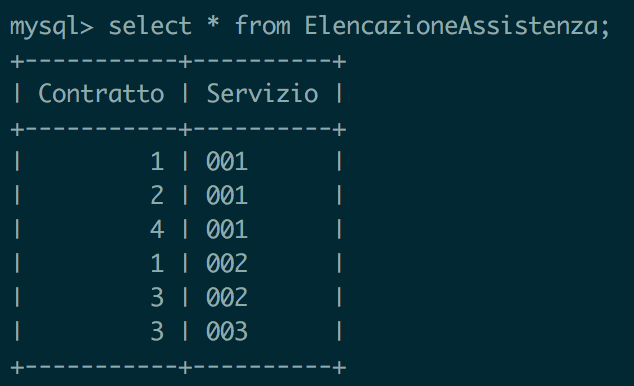
\includegraphics[width=0.7\linewidth]{./immagini/20}}
\newline\newline

\begin{verbatim}
create table DescrizioneRichiesta (
  RichiestaMEPA INT(11),
  ProdottoServizio VARCHAR(20),
  Quantita INT(11) not null default 1,
  primary key (RichiestaMEPA, ProdottoServizio),
  foreign key (RichiestaMEPA) references RichiestaMEPA(Numero)
    on update cascade on delete no action,
  foreign key (ProdottoServizio) references ProdottoServizio(Codice)
    on update cascade on delete no action
)ENGINE=InnoDB;
\end{verbatim}
\vspace{0.5cm}

\noindent\makebox[\textwidth]{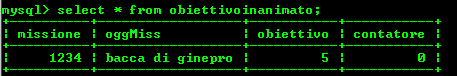
\includegraphics[width=0.7\linewidth]{./immagini/21}}
\newline\newline

\begin{verbatim}
create table Acquisto (
  Fattura INT(11),
  Prodotto VARCHAR(20),
  primary key (Fattura, Prodotto),
  Quantita INT(11) not null default 1,
  foreign key (Fattura) references Fattura(Codice)
    on update cascade on delete no action,
  foreign key (Prodotto) references Prodotto(Codice)
    on update cascade on delete no action
)ENGINE=InnoDB;
\end{verbatim}
\vspace{0.5cm}

\noindent\makebox[\textwidth]{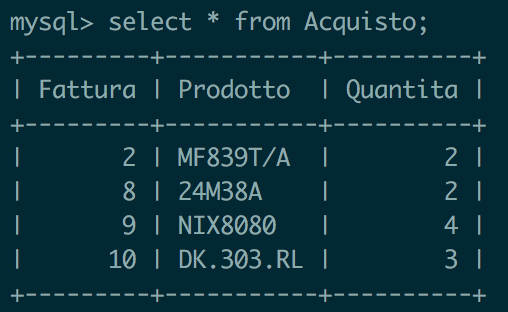
\includegraphics[width=0.5\linewidth]{./immagini/22}}
\newline\newline

\begin{verbatim}
create table Vendita (
  Fattura INT(11),
  ProdottoServizio VARCHAR(20),
  primary key (Fattura, ProdottoServizio),
  Quantita INT(11) not null default 1,
  foreign key (Fattura) references Fattura(Codice)
    on update cascade on delete no action,
  foreign key (ProdottoServizio) references ProdottoServizio(Codice)
    on update cascade on delete no action
)ENGINE=InnoDB;
\end{verbatim}
\vspace{0.5cm}

\noindent\makebox[\textwidth]{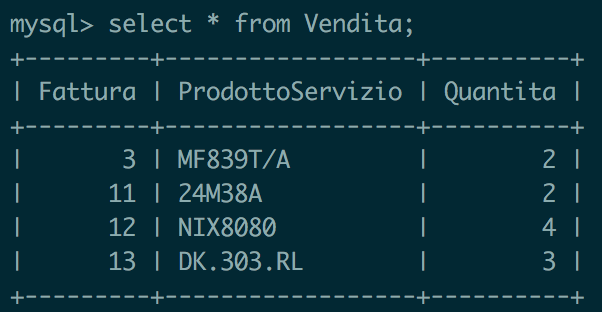
\includegraphics[width=0.6\linewidth]{./immagini/23}}
\newline\newline
